\subsection{Accumulator Concept}

\ifCommentInclude
%%%%%%%%%%%%%%%%%%%%%%%%%%%%%%%%%%%%%%%%%%%%%%%%%%%%%%%%%%
\begin{frame}[t]{Accumulator Concept}
    \justifying
    
    \begin{figure}[htpb]
        \centering
        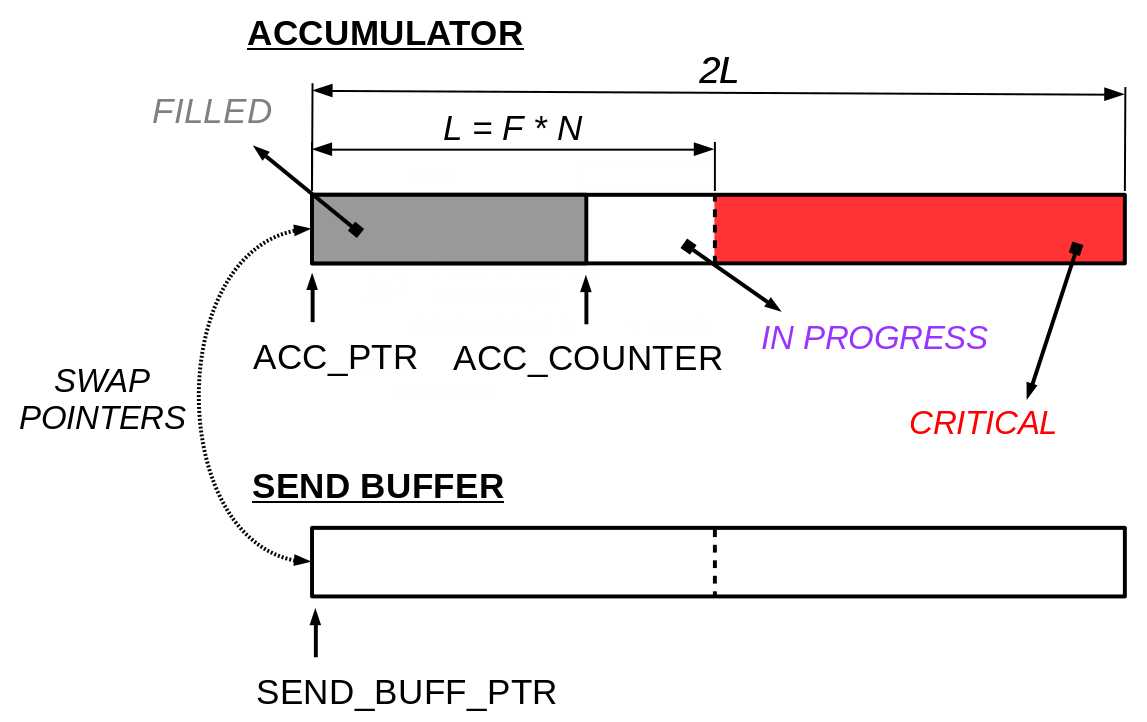
\includegraphics[width=0.8\textwidth]{figures/chapter-3/accumulator-concept.png}
        \caption{Accumulator concept} \label{fig:accumulator-concept}
    \end{figure}

\end{frame}
\fi

%%%%%%%%%%%%%%%%%%%%%%%%%%%%%%%%%%%%%%%%%%%%%%%%%%%%%%%%%%
\begin{frame}[t]{Accumulator Concept}
    \justifying
    \begin{columns}
    \column{0.5\textwidth}
        \begin{figure}[t]
            \centering
            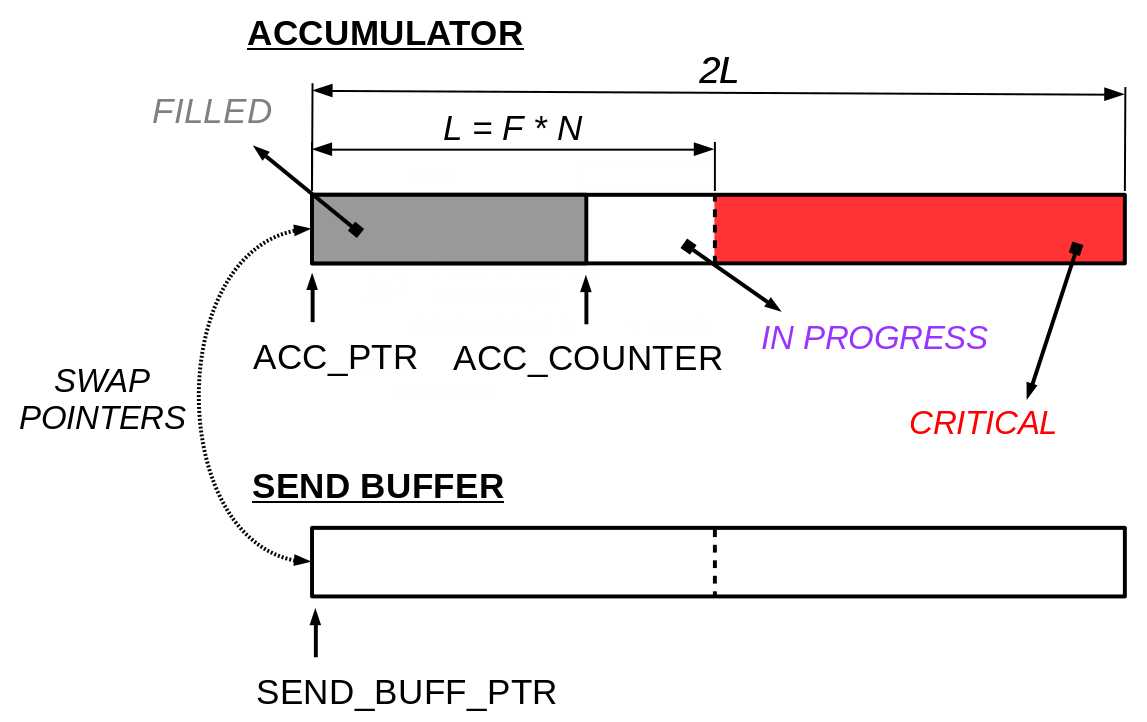
\includegraphics[width=0.9\textwidth]{figures/chapter-3/accumulator-concept.png}
        \end{figure}
    \column{0.5\textwidth}
        \begin{figure}[t]
            \centering
            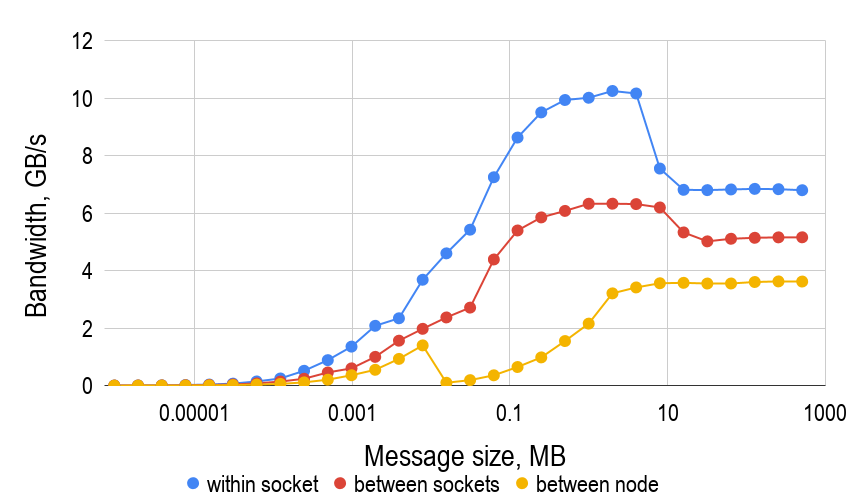
\includegraphics[width=0.9\textwidth]{figures/chapter-3/hw1-bandwidth.png} \label{fig:hw1-bandwidth}
        \end{figure}
    \end{columns}
    
    \spc
    Accumulator concept allows to:
    \begin{itemize}
        \item enable \textbf{non-blocking} data transfer
        \item \textbf{reduce} the number of client \textbf{requests} i.e. handshakes, resource acquisitions
        \item achieve \textbf{full bandwidth} utilization
        
    \end{itemize}

\end{frame}

%%%%%%%%%%%%%%%%%%%%%%%%%%%%%%%%%%%%%%%%%%%%%%%%%%%%%%%%%%
\begin{frame}[t]{Example:  N = 100; F = 1}
    \small
    \justifying
    \begin{itemize}
        \item The original \textbf{distribution shape} is transformed to the \textbf{rectangular} one
        \item Data is transferred in \textbf{equal chunks}
    \end{itemize}
    
    
    \begin{figure}[t]
        \centering
	    \begin{tabular}{cc}
		    \subfloat[Before]{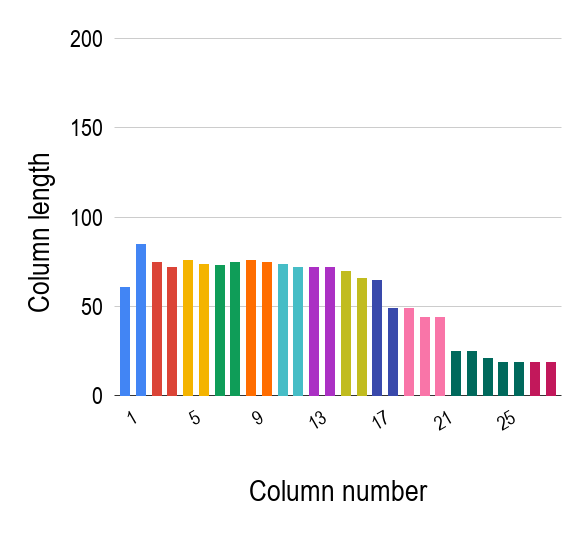
\includegraphics[width=0.42\textwidth]{figures/chapter-3/accumulation-before.png}} &
		    \subfloat[After]{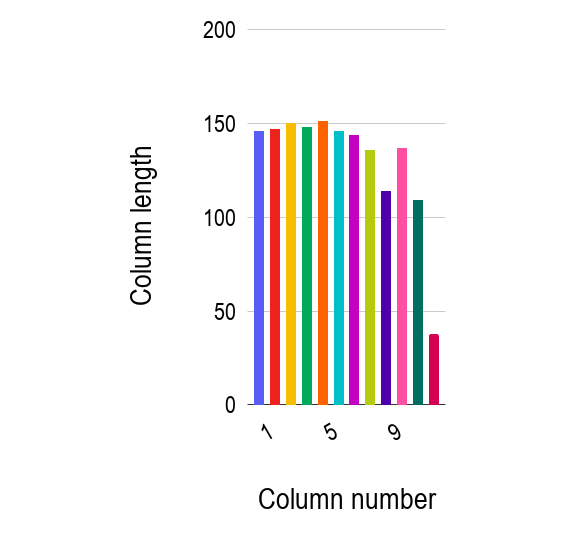
\includegraphics[width=0.42\textwidth]{figures/chapter-3/accumulation-after.png}} \\
	        \end{tabular}
	\label{fig:accumulator-in-action}
    \end{figure}

\end{frame}